\documentclass[12pt]{article}
\usepackage{graphicx, amsmath}
\usepackage{caption}
\usepackage{algorithm}
\usepackage{algpseudocode}
\graphicspath{ {./} }
\setlength{\oddsidemargin}{0.25 in}
\setlength{\evensidemargin}{-0.25 in}
\setlength{\topmargin}{-0.6 in}
\setlength{\textwidth}{6.5 in}
\setlength{\textheight}{8.5 in}
\setlength{\headsep}{0.75 in}
\setlength{\parindent}{0 in}
\setlength{\parskip}{0.1 in}

\begin{document}
\thispagestyle{plain}
   \newpage
   \setcounter{page}{1}
   \noindent
   \begin{center}
   \framebox{
      \vbox{\vspace{2mm}
    \hbox to 6.28in { {\bf BioE 131: Intro to Computational Biology}
                        \hfill Fall 2020 }
       \vspace{4mm}
       \hbox to 6.28in { {\bf \Large \hfill Biological Ontologies  \hfill} }
       \vspace{2mm}
       \hbox to 6.28in { {\it Professor: Ian Holmes \hfill} }
      \vspace{2mm}}
   }
   \end{center}
   {Notes written by Vikram Shivakumar}
   \vspace*{4mm}


\section{Introduction}
In this note, we'll take a look at \textbf{ontologies}, specifically biological ontologies. An ontology is a \textit{formal} representation of categories, items, and relations using a controlled vocabulary. For example, if we are interested in genes related to terpene biosynthesis (an organic compound with a strong odor), one way to compile a list of genes would be to search all previous publications for genes involved in the pathway. But sometimes naming conventions can differ, so we have to try multiple variants of the same search term. Also, once we get the names of genes, we need to do more searching to find the relevant sequences!\\[10pt]
An ontology addresses this problem by assigning this category a standard name (``terpenoid biosynthetic process"). Then we can search for all genes related to this standard search term and find all the genes of interest!

\section{Ontologies}
There are a few different ontologies in biology. An important one is the \textbf{Gene Ontology}, which describes genes, gene function, and biological processes using \textbf{GO terms}. Other ontologies exist for biological fields like disease, anatomy, biochemistry, etc.
\subsection{Gene Ontology}
The Gene Ontology (GO) contains $\sim50,000$ terms, split into three main categories. \textbf{Molecular function} terms describe tasks or activities performed by a gene product, for example ``catalysis" or ``receptor binding". \textbf{Biological process} terms describe broader processes like ``mitosis" or ``DNA replication". Lastly, \textbf{cellular component} terms describes a location like ``cytoplasm" or ``telomere" which is related to a gene.\\[10pt]
From the description of the three main cateogries, it is clear that a given gene can be associated with multiple GO terms across the ontology. For example, a single gene can have multiple functions, or a single function involved in multiple biological processes, acting in various cellular components.
\subsection{Ontology relationships}
GO terms can be very broad (``biosynthetic process") to very specific (``monoterpenoid biosynthetic process"), and so relationships between terms naturally arise. The nature of these relationships is in and of itself another ontology (OBO relations ontology, e.g. ``is\_a", ``part\_of", etc.) The relationships between terms can be modeled by a \textbf{Directed Acyclic Graph (DAG)}.

\section{Term Enrichment Analysis}
Suppose we run an RNA-seq experiment and collect a list of genes which we find are expressed in a tissue of interest. We can annotate this list of expressed genes with GO terms. One question we can ask is if a GO term is \textbf{enriched}, or over represented in this list of genes.

\subsection{Hypergeometric test}
A \textbf{hypergeometric distribution} can be used to answer this question. Assume there are $N$ genes total in the genome, of which $m$ genes are annotated with a specific GO term $Y$. In our experiment, we find $n$ genes, of which $k$ are annotated with GO term $Y$. 
\begin{figure}[h!]
    \centering
    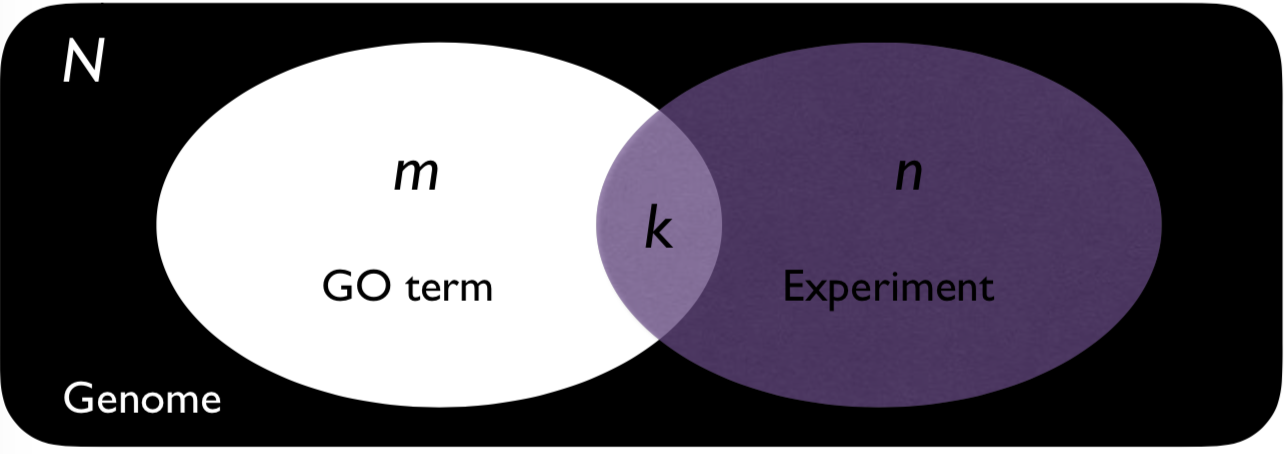
\includegraphics[width = .6\linewidth]{enrich.png}
    \caption{Venn diagram of a hypothetical GO term enrichment scenario}
    \label{fig:my_label}
\end{figure}

What is the probability that these $k$ genes are annotated? We can use the hypergeometric distribution to find this probability and evaluate if this result is significant:
$$P(X = k) =  \frac{\binom{m}{k} \binom{N-m}{n-k}}{\binom{N}{n}}$$
Recall that the \textbf{binomial coefficient} $\binom{A}{B}$ represents the number of ways to choose a subset $B$ items from a set of $A$ items.\\[10pt]
The first term $\binom{m}{k}$ represents the number of ways to choose $k$ genes from the set of genes with GO term $Y$. Next, $\binom{N-m}{n-k}$ represents the number of combinations to choose the remaining $n-k$ genes from the set of genes that are NOT annotated with GO term $Y$. Lastly, we normalize the probability by the number of ways to select the $n$ genes in our list from the total number of genes $N$.\\[10pt]
Lastly, we can find the probability of $k$ \textit{or more} genes annotated with GO term $Y$, $P(X\geq k)$, by integrating over the tail of the distribution. This probability is the $p$-value for the one-tailed \textbf{Fisher's Exact Test}. 

\subsection{Multiple Test correction}
After running a Fisher's exact test, assume we get a $p$-value of $0.001$. We can interpret this value as the probability that this result occurred by chance. What if we run this statistical test on 1,000 GO terms? Then if this result occurs by chance with probability $p = 0.001$, after 1,000 tests, we can expect that one of the test results happened by chance!\\[10pt]
To correct for running multiple tests, we can use the \textbf{Šidák correction}. When running many tests, we want to find the probability that at least one of the tests is significant:
$$P(\text{at least 1 test significant})$$
$$1 - P(\text{none significant})$$
$$1 - (1 - \beta)^n$$
where $\beta$ is the threshold for significance for each test, and $n$ is the number of tests run. $1-\beta$ is the probability that a result was not by chance, and thus $(1-\beta)^n$ is the probability that \textit{all} $n$ results are not by chance. We can set a threshold for this probability at $\alpha$, and solving for $\beta$, we get:
$$\beta = 1 - (1 - \alpha)^\frac{1}{n}$$
Thus if we want an overall significance of $\alpha = 0.05$ (probability of at least 1 significant test is $0.05$), then we need to set a significance threshold $\beta = 1 - (0.95)^\frac{1}{n}$ for each individual test. \textit{Note}: this correction is conservative, since it assumes each test is independent (not necessarily true, since GO terms are related).

\subsection{Binomial Test}
Another similar approach (Bejerano \textit{et al}, 2010) uses the binomial distribution (see the note on Probability). Assume again that of $n$ expressed genes, $k$ are annotated with term $Y$. Now assume that a proportion $p_Y$ of the genome is annotated with $Y$. We get the following probability:
$$P(X = k) = \binom{n}{k}p_Y^k(1 - p_Y)^k$$
Again, we can take the sum over the tail of the binomial distribution to find the probability $P(X\geq k)$.\\[10pt]
This binomial test represents a scenario where we can select items from the set of gene annotated with term $Y$ \textit{with replacement}. This differs from the hypergeometric test, where we sample from the set of genes \textit{without replacement}.

\subsection{Bayesian term enrichment}
The previous statistical tests are \textbf{frequentist significance tests}. Another method for analyzing term enrichment uses Bayesian techniques, specifically building a \textbf{Bayes net} that models the set of terms that \textit{best} explain the activated gene set.
\begin{figure}[h]
    \centering
    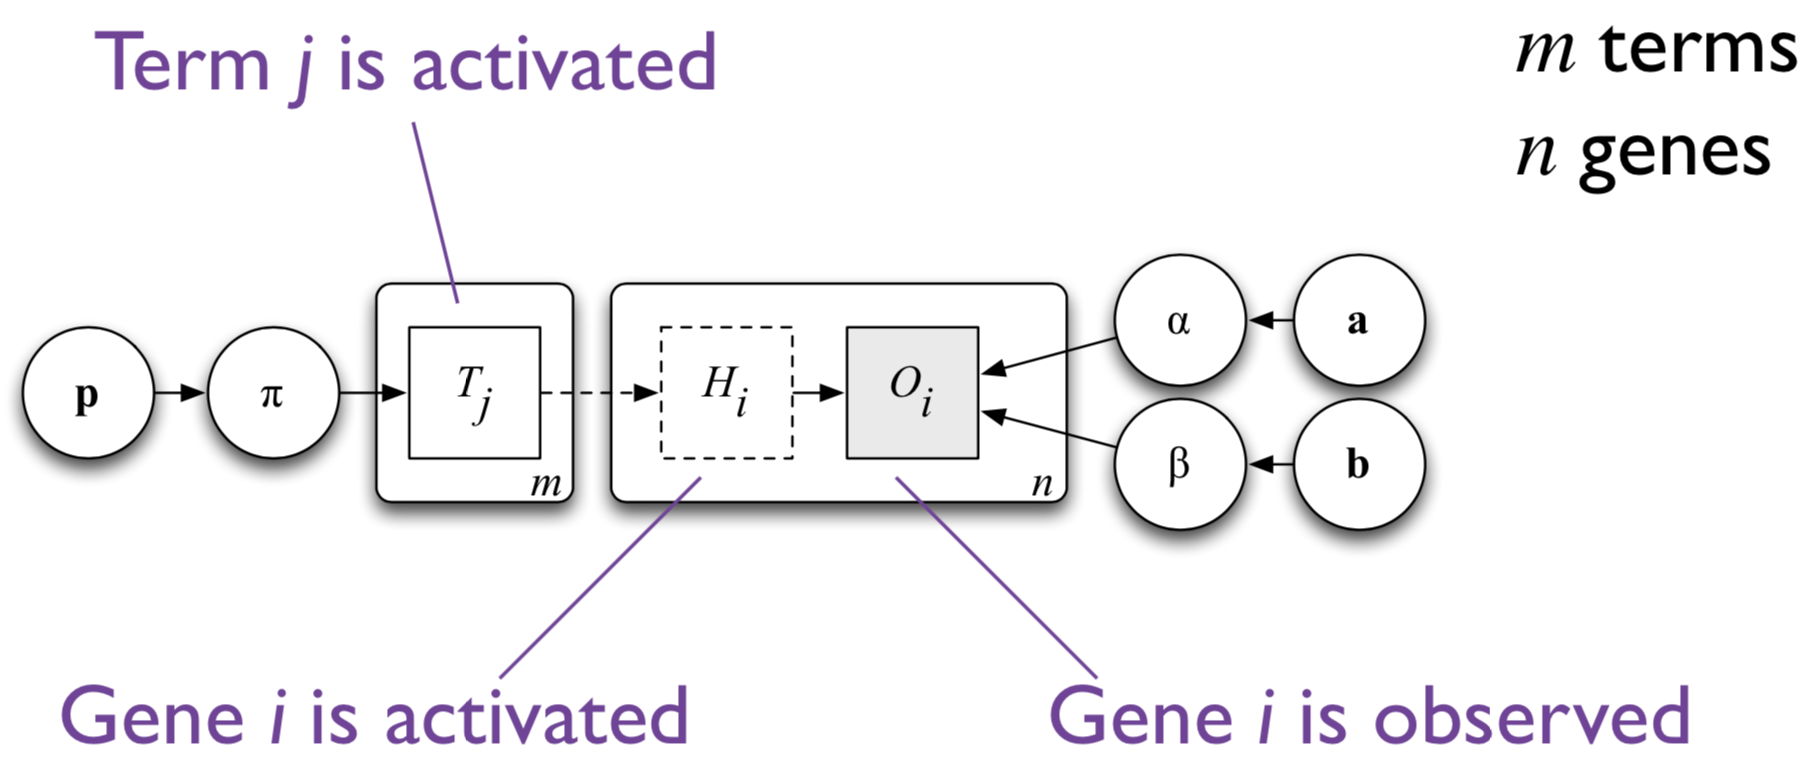
\includegraphics[width=.8\linewidth]{bayes.png}
    \caption{A Bayes net to model term enrichment}
    \label{fig:bayes}
\end{figure}

Figure \ref{fig:bayes} shows a type of Bayes net, where $T_j$ represents GO term $j$, $H_i$ represents the \textit{hidden state} of gene $i$ and $O_i$ the \textit{observed state}. Since we assume that gene activation is \textit{noisy}, i.e there is a probability $\alpha$ of a false positive and $\beta$ of a false negative, the true state of activation is modeled by the hidden state (which we can only infer from the observation). Lastly in order to complete the model, we define $\pi$, the prior probability of each term being activated.\\[10pt]
Often the Bayes net is used in an \textbf{MCMC sampler}, which iteratively makes changes to the states of the graph, mostly towards more likely states, but sometimes to less likely ones as well. Some ``moves" in this type of network include: activating/deactivating a random term, swapping a term with a random or related term, or randomly sampling all terms. After many iterations, we can find the most likely set of activated terms given a set of observed genes (see note on Probability and RNA folding for Bayes nets and MCMC sampling).

\section{Summary}
Ontologies can create a standard set of terms to integrate research across the field of biology. They can be useful in bioinformatics to assign functional terms to sequenced genes, analyze the relationships between biological processes, and determine if broader processes or pathways are represented by a set of genes. Lastly, this task of term enrichment can be approached with various probabilistic methods like frequentist and Bayesian statistics.

\end{document}


%topics not covered:
